%%%%%%%%%%%%%%%%%%%%%%%%%%%%%%%%%%%%%%%%%%%%%%%%%%%%%%%%%%%%%%%%%%%%%
%
%  This is a sample LaTeX input file for your contribution to 
%  the MC2013 conference. Modified by R.C. Martineau at INL from A. 
%  Sood at LANL, from J. Wagner ORNL who obtained the original class 
%  file by Jim Warsa, LANL, 16 July 2002}
%
%  Please use it as a template for your full paper 
%    Accompanying/related file(s) include: 
%       1. Document class/format file: mc2013.cls
%       2. Sample Postscript Figure:   figure.eps
%       3. A PDF file showing the desired appearance: template.pdf 
%    Direct questions about these files to: richard.martinea@inl.gov
%
%    Notes: 
%      (1) You can use the "dvips" utility to convert .dvi 
%          files to PostScript.  Then, use either Acrobat 
%          Distiller or "ps2pdf" to convert to PDF format. 
%      (2) Different versions of LaTeX have been observed to 
%          shift the page down, causing improper margins.
%          If this occurs, adjust the "topmargin" value in the
%          mc2013.cls file to achieve the proper margins. 
%
%%%%%%%%%%%%%%%%%%%%%%%%%%%%%%%%%%%%%%%%%%%%%%%%%%%%%%%%%%%%%%%%%%%%%


%%%%%%%%%%%%%%%%%%%%%%%%%%%%%%%%%%%%%%%%%%%%%%%%%%%%%%%%%%%%%%%%%%%%%
\documentclass{mc2013}
%
%  various packages that you may wish to activate for usage 
\usepackage{graphicx}
\usepackage{tabls}
\usepackage{afterpage}
\usepackage{float}
\usepackage{cites}
\usepackage{color}
\usepackage{amsmath,amsthm,amssymb}
\usepackage{verbatim}
\usepackage[parfill]{parskip}
\usepackage{tikz}
\usepackage{subcaption}
\usepackage{soul}
\usepackage[labelfont=bf]{caption}
\usepackage[framemethod=tikz]{mdframed}
 
\renewcommand{\thefootnote}{\fnsymbol{footnote}}
\newcommand{\N}{\mathbb{N}}
\newcommand{\Z}{\mathbb{Z}}
\newcommand{\deriv}[2]{\frac{\mathrm{d} #1}{\mathrm{d} #2}}
\newcommand{\pderiv}[2]{\frac{\partial #1}{\partial #2}}
\newcommand{\bx}{\mathbf{X}}
\newcommand{\ba}{\mathbf{A}}
\newcommand{\by}{\mathbf{Y}}
\newcommand{\bj}{\mathbf{J}}
\newcommand{\bs}{\mathbf{s}}
\newcommand{\B}[1]{\ensuremath{\mathbf{#1}}}
\newcommand{\Dt}{\Delta t}
\renewcommand{\d}{\mathrm{d}}
\newcommand{\mom}[1]{\langle #1 \rangle}
\newcommand{\cur}[1]{\left\{ #1 \right\}}
\newcommand{\xl}{{x_{i-1/2}}}
\newcommand{\xr}{{x_{i+1/2}}}
\newcommand{\il}{{i-1/2}}
\newcommand{\ir}{{i+1/2}}
\newcommand{\jl}{{j-1/2}}
\newcommand{\jr}{{j+1/2}}

\graphicspath{{figures/}}
 
%\usepackage{epsf}
%
%
% Insert authors' names and short version of title in lines below
%
\newcommand{\authorHead}      % Author's names here
   {S.R. Bolding, M. Cleveland, and J.E. Morel}  
\newcommand{\shortTitle}      % Short title here
   {A HOLO method with ECMC for Thermal Radiative Transfer}  
%%%%%%%%%%%%%%%%%%%%%%%%%%%%%%%%%%%%%%%%%%%%%%%%%%%%%%%%%%%%%%%%%%%%%
%
%   BEGIN DOCUMENT
%
%%%%%%%%%%%%%%%%%%%%%%%%%%%%%%%%%%%%%%%%%%%%%%%%%%%%%%%%%%%%%%%%%%%%%
\begin{document}

%
%      Headers and Footers
\afterpage{%
\fancyhf{}%
\fancyhead[CE]{              
{\scriptsize \authorHead}}                                                
\fancyhead[CO]{               
{\scriptsize \shortTitle}}                  
%\lfoot{\scriptsize{
%International Conference on Mathematics and Computational Methods
%Applied to Nuclear Science \& Engineering (M\&C 2013), 
%\\ Sun Valley, Idaho, USA, May 5-9, 2013.}}%
\rfoot{\thepage/\totalpages{}}%

\pagestyle{fancy}
%\setlength{\topmargin}{-20pt}
}

\renewcommand\thesection{\Roman{section}}
\renewcommand\thesubsection{\thesection.\Alph{subsection}}
 
\normalsize
\setlength{\baselineskip}{16.8pt}
\vspace{-3pt}

% 
% TITLE
%

\begin{center}
\textbf{\large \\%
A HIGH-ORDER LOW-ORDER ALGORITHM WITH EXPONENTIALLY-CONVERGENT MONTE CARLO FOR
THERMAL RADIATIVE TRANSFER\\ \vspace{0.1in}
}
% 
% FIRST AUTHORS 
%
\setlength{\baselineskip}{14pt}
\textbf{Simon R. Bolding\footnote{LA-UR-14-29653} and Jim E. Morel} \\
Department of Nuclear Engineering\\
Texas A\&M University  \\
College Station, TX 77843 \\
sbolding@tamu.edu; morel@tamu.edu \\

% 
% SECOND AUTHORS (if not needed delete from here) 
%
\vspace{6.2pt}
\textbf{Mathew A. Cleveland}\\
Los Alamos National Laboratory \\
Los Alamos, NM 87545 \\
cleveland@lanl.gov \\ 
%
% SECOND AUTHORS (to here)
%

\end{center}

%
% SET RAGGED RIGHT MARGIN
%
\raggedright

\vspace{4pt}
\section*{ABSTRACT} 
\begin{quote}
\begin{small}
We have implemented a new high-order low-order (HOLO) algorithm for solving
thermal radiative transfer problems.  The low-order (LO) system is based on spatial
and angular moments of the transport equation and a linear-discontinuous
finite-element spatial representation, producing equations similar to the standard
S$_2$ equations.  
The LO solver is fully implicit in time and efficiently resolves the non-linear
temperature dependence at each time step.   The HO solver
utilizes exponentially-convergent Monte Carlo (ECMC) to give a globally accurate solution
for the angular intensity to a fixed-source, pure absorber transport problem.  This global solution is used to compute consistency terms
that require the HO and LO solutions to converge towards the same solution.  The use of ECMC
allows for the efficient reduction of statistical noise in the MC solution, reducing
inaccuracies introduced through the LO consistency
terms.  We compare results with an
implicit Monte Carlo (IMC) code for one-dimensional, gray test problems and 
demonstrate the efficiency of ECMC over standard Monte Carlo in this algorithm.

\emph{Key Words}: hybrid Monte Carlo, residual Monte Carlo, thermal radiative transfer

\end{small} 
\end{quote}

\setlength{\baselineskip}{14pt}
\normalsize

\Section{INTRODUCTION}

We have implemented a high-order low-order (HOLO) algorithm for the case of 1D gray thermal radiative transfer (TRT) problems. The governing equations are the radiation and
material energy balance equations, i.e.,\vspace{-0.05in}
\begin{align}\label{ho_cont}
    \frac{1}{c}\pderiv{I}{t} + \mu \pderiv{I}{x} + \sigma_t I
&= \frac{\sigma_s}{2} \phi +\frac{1}{2} \sigma_a a c T^4
    \\ \label{t_cont}
  \rho c_v \pderiv{T}{t} &=  \sigma_a \phi - \sigma_a a c T^4.
\end{align}
In the above equations $x$ is the position, $t$ is the time, $\mu$ is
the $x$-direction cosine of the angular intensity $I(x,\mu,t)$, and $a$, $c$, $\rho$,
and
$c_v$ are the radiation constant, speed of light, mass density, and specific heat; $\sigma_a$, $\sigma_s$, and
$\sigma_t$ are the absorption, scattering, and total
cross sections (cm$^{-1}$), respectively. The desired unknowns are the material
temperature $T(x,t)$ and the scalar radiation intensity $\phi(x,t)=\int_{-1}^1
I(x,\mu,t) \d \mu$. The equations are
strongly coupled through the gray Planckian emission source $\sigma_a a c T^4$, which
is a nonlinear function of temperature, and the absorption
term $\sigma_a \phi$.   In general, the material properties are a function of $T$.  The temperature dependent material properties and
absorption- reemission physics lead to systems that require solution in a mix of
streaming and optically-thick, diffusive regions. 

Monte Carlo (MC) solution to the TRT equations is typically achieved by the 
implicit Monte Carlo (IMC) method~\cite{fnc}. This
method linearizes Eq.~\eqref{ho_cont} \& Eq.~\eqref{t_cont} over a discrete time
step.  The linearization of the system produces a transport equation that contains an approximate emission source and an effective scattering cross section representing
absorption and reemission of photons over a time step. This transport equation is solved using MC. The MC simulation tallies energy absorption
over a discretized spatial mesh.  The energy absorption in each mesh cell is used to directly estimate
a new end of time step temperature in that cell.  In optically thick regions, or for
large time steps, the
effective scattering dominates interactions.  In these diffusive regions IMC
becomes computationally expensive. Acceleration methods typically attempt to improve
efficiency by allowing particles to take discrete steps through optically thick
regions based on a discretized diffusion approximation~\cite{imd,ddmc}. In IMC the
approximate linearization of the emission source is not iterated on within a time
step due to the large computational cost of the MC transport each time step; this
imposes a limit on the time step size to produce physically accurate
results~\cite{wollaber2013discrete}. 

Moment-based hybrid Monte Carlo (MC) methods provide an alternative solution method.
Recent work has focused on so-called high-order low-order (HOLO)
approaches~\cite{willert,park,rmc,ans_2014}.  Such methods utilize a low-order (LO)
operator based on angular moments of the transport equation, formulated over a fixed
spatial mesh. Physics operators that are time consuming for MC
to resolve, e.g., absorption-reemission and scattering events, are moved to the LO
system.  Newton methods allow for non-linearities in the LO equations to be fully
resolved efficiently~\cite{willert}.  The high-order (HO) transport equation is defined by 
Eq.~\eqref{ho_cont}, with sources that are truly implicit in time estimated from the LO solution. The HO equation is solved via MC to produce a high-fidelity solution for
the angular intensity.  The MC estimate of the angular intensity is used to estimate consistency terms,
present in the LO equations, that require the LO system to preserve the angular accuracy of the
MC solution.  The HO system does not directly estimate a new material temperature,
eliminating stability issues that require linearization of the emission source.

Sufficient MC histories must be performed to eliminate statistical
noise in the consistency terms that can contaminate the LO solution.
Exponentially-convergent Monte Carlo (ECMC)\cite{ecmc} provides an algorithm that can efficiently
reduce statistical noise to the same order as the HOLO iteration error with
significantly less particle histories than standard MC. In particular, ECMC is
exceptionally efficient in time-dependent TRT problems because information about the
intensity from the previous time step can be used as an accurate initial guess for
the end of time step intensity. Additionally, no particle histories are required in regions of the problem
where the problem is in equilibrium, similar to~\cite{rmc}.  However, implementation
of ECMC is non-trivial, requiring a finite-element representation of the solution in all
phase-space variables.  The fundamental transport of particles is the same
as standard Monte Carlo transport codes, but the source will now contain positive and
negative weight particles.

Our ECMC solver contains similarities to the residual Monte Carlo (RMC) HO solver
in~\cite{rmc}, with some key differences.  The RMC algorithm uses a particular, fixed 
estimate of the solution to significantly reduce the statistical noise in the
simulation compared to a standard MC simulation. The guess for the solution is chosen to produce only sources on the faces of
cells, reducing the dimension of the phase-space to be sampled~\cite{rmc}. The RMC
algorithm  uses a piecewise constant trial space representation for the intensity in
$x$ and $\mu$.
The primary difference between the methods is that ECMC iteratively estimates the
solution, in batches, producing a known MC estimate
of the error in that estimate.  The ECMC algorithm also uses a linear-discontinuous
finite-element (LDFE) trial space to represent the intensity, although the RMC
algorithm could similarly be formulated with an LDFE representation.  The LDFE
representation introduces significant implementation complexity.  The formulation of the residual in~\cite{rmc} can produce minimal
statistical noise in slowly varying problems where the behavior of the system is near
equilibrium. The ECMC algorithm has
similar statistical efficiency by choosing the old intensity as the initial guess to
the algorithm.  The ECMC algorithm will generally be more efficient in cases where
the solution varies greatly over a time step or when very low statistical noise is
desired.  Generally, the minimum number of histories per batch to obtain convergence with the
LDFE trial space is larger than a piece-wise constant representation because additional
histories are needed to sufficiently estimate the first moment in $x$ and $\mu$ of the
intensity. It is noted that our formulation of the LO
equations is in great contrast to the formulation in~\cite{rmc}.

In this work, we demonstrate the utility of an S$_2$-like LO operator~\cite{wolters}
in conjunction with an ECMC method~\cite{jake} for the HO solver.
The ECMC algorithm uses information about the intensity from the previous time step to reduce statistical noise to the same order as
the HOLO iteration error with significantly less particle histories than standard MC
simulations, with less computational cost than IMC per history.  We have derived the LO operator directly from the transport
equation, using a linear-discontinuous (LD) finite-element (FE) spatial
discretization, such that the HO and LO solutions are converging towards the same
solution.
Herein we describe the algorithm and present results for two??? test problems.

\Section{Overview of the HOLO Algorithm}

For simplicity, our HOLO method will use a backwards Euler discretization in time, as
well as constant specific heats and cell-wise constant opacities. The time discretized
equations are
\begin{align}
\mu \pderiv{I^{n+1}}{x} + \left(\sigma_t + \frac{1}{c \Delta t }\right) I^{n+1}
&= \frac{\sigma_s}{2} \phi^{n+1} +\frac{1}{2} \left(\sigma_a a c T^4 \right)^{n+1} + \frac{I^n}{c \Delta t} \label{ho_trans} \\
\rho c_v \frac{T^{n+1} - T^n}{\Delta t} &= \sigma_a \phi^{n+1}
- \sigma_a a c (T^4)^{n+1} \label{lo_mat}.
\end{align}
where $\Delta t$ is the time step size and the superscript $n$ is used to indicate
the $n$-th time step. It is noted that in IMC the time derivative in
Eq.~\eqref{ho_cont} is typically treated using continuous time-dependent MC over each
time step.  Our HO transport equation is
discrete in time for easy application of ECMC and to avoid difficulties in coupling to the
fully-discrete LO solver, but this does introduce some artificial propagation of
energy due to the implicit time differencing, in optically thin regions. 

In the HOLO context, the LO solver models the physical scattering and
resolves the material temperature spatial distribution $T(x)$ at each time step.  The LO equations are formed via half-range 
angular and spatial moments of
Eq.~\eqref{ho_trans} and Eq.~\eqref{lo_mat}, formed over a spatial finite element
mesh.  The angular treatment in the LO equations has the same form as those used in the
hybrid-S$_2$ method in~\cite{wolters},  with
element-averaged consistency parameters that are analogous to a variable
Eddington factor.  If the angular consistency parameters were estimated exactly, then the LO equations are exact with respect to the chosen
spatial discretization.  These consistency parameters are lagged in each LO solve,
estimated from the previous HO solution for $I^{n+1}(x,\mu)$, as explained below. For
the initial LO solve for each time step, the parameters are calculated based on the
$I^{n}(x,\mu)$.  The LO equations always conserve total energy, independent of the accuracy of the consistency terms.

The solution to the LO system is used to construct a spatially LD representation of
the scattering and emission sources on the right hand side of Eq.~\eqref{ho_trans}.  This defines a fixed-source, pure absorber
transport problem for the HO operator. This HO transport problem represents a characteristic method that uses MC to
invert the continuous streaming plus removal operator with an LD representation of
sources. We will solve this transport problem using ECMC.  The output from ECMC is
$\tilde{I}(x,\mu)$, a space-angle LDFE projection of the exact solution for
$I(x,\mu)$.  Once computed, $\tilde{I}(x,\mu)$ is used
to directly evaluate the necessary consistency parameters for the next LO solve.  Since there is a global, functional representation of
the angular intensity,  LO parameters are estimated using quadrature and do not
require additional tallies.  The HO solution is not used to directly estimate a new
temperature at the end of the time step; it is
only used to estimate the spatial and angular parameters in the LO solution, which eliminates
typical operator splitting stability issues that require linearization of the emission source.

The process of performing subsequential HO and LO solves, within a single time step, can be repeated to obtain an increasingly accurate solution for $\phi^{n+1}(x)$ and $T^{n+1}(x)$.  Thus, the HOLO algorithm, for the $n$-th time step, is
\begin{enumerate}
\item Perform a LO solve to produce an initial guess for $T^{n+1,0}(x)$
    and $\phi^{n+1,0}(x)$, based on consistency terms estimated with $\tilde{I}^{n}$.
\item Solve the HO system for $\tilde{I}^{n+1,k+1/2}(x,\mu)$ using ECMC, based on the current
    LO estimate of the emission and scattering sources.%$\sigma_s(T^k)\phi^{k}$ and $B(T)^{k}$.
\item Compute LO consistency parameters with $\tilde{I}^{n+1,k+1/2}$.  
\item Solve the LO system using HO consistency parameters to produce a new
    estimate of $\phi^{n+1,k+1}$ and $T^{n+1,k+1}$.
\item Repeat 2 -- 4 until convergence is achieved.
\item Store $\tilde{I}^{n}\leftarrow\tilde{I}^{n+1}$, and move to the next time step.
\end{enumerate}
where the superscript $k$ denotes an outer HOLO iteration.
The consistency terms force the HO
and LO solutions for $\phi^{n+1}(x)$ to be consistent to the order of the current HOLO
iteration error.
%One HOLO fixed-point iteration $k$ denotes the process of an ECMC solve of the HO problem to estimate LO parameters, based on
%the current LO estimate of sources, followed by a solution of the 
%LO system for $T^{n+1}(x)$ and $\phi^{n+1}(x)$.


\Section{Forming the Low-Order System}

To form the LO system of equations, spatial moments are taken over each spatial cell $i$:
$x\in[x_{i-1/2},x_{i+1/2}]$, weighted with the standard linear FE
interpolatory basis functions.  For example, the $L$  moment operator is defined by
\begin{equation}\label{x_mom}
\mom{\cdot}_{L,i} = \frac{2}{h_i} \int_{x_{i-1/2}}^{\xr} b_{L,i}(x) (\cdot) \d x,
\end{equation}
where $h_i=x_{i+1/2}-x_{i-1/2}$ is the width of the spatial element and
$b_{L,i}(x)=(x_{i+1/2}-x)/h_i$ is the FE basis function, for cell $i$, corresponding to position
$x_{i-1/2}$.  The right moment $\mom{\cdot}_R$ is defined with weight function $b_{R,i}(x)=(x -
x_{i-1/2})/h_i$. Here, it is noted in this notation that $\mom{\phi}_{L,i}$ and
$\mom{\phi}_{R,i}$ represent spatial moments of the intensity over cell $i$, rather
than $\phi_{L,i}$ and $\phi_{R,i}$ which represent the interior value of the linear
$\phi(x)$ at $x_\il$ and $x_\ir$. To reduce the angular dimensionality, positive and
negative half-range integrals of the angular intensity are taken.  The half-range
averages of $I$ are defined as $ \phi^+(x) = \int_0^{1} I(x,\mu) \d \mu$ and $ \phi^-(x) = \int_{-1}^{0} I(x,\mu) \d
\mu$, respectively.  Thus, in terms of half-range quantities, $\phi(x) = \phi^-(x) +
\phi ^+(x)$.  

\Subsection{Radiation Energy Equations}

Pairwise application of the $L$ and $R$ basis
moments with the $+$ and $-$ half-range integrals to Eq.~\eqref{ho_trans} 
ultimately yields four radiation moment
equations per cell. As in~\cite{wolters}, algebraic manipulation is performed to form
intensity-weighted
averages of $\mu$, which we call consistency terms.  As an example, the final equation resulting from application of the $L$ moment and
positive half-range integral is
\begin{multline}\label{lo_tran}
    -2{\mu}_{i-1/2}^{n+1,+} \phi_{i-1/2}^{n+1,+} + \cur {\mu}_{L,i}^{n+1,+}
  \mom{\phi}_{L,i}^{n+1,+}
  +  \cur\mu_{R,i}^{n+1,+}
  \mom{\phi}_{R,i}^{n+1,+} +  \left(\sigma_t^{n+1}+\frac{1}{c \Delta t} \right) h_i 
  \mom{\phi}_{L,i}^{n+1,+} \\-  \frac{\sigma_s h_i}{2} \left( \mom{\phi}_{L,i}^{n+1,+} +
  \mom\phi_{L,i}^{n+1,-}\right) = \frac{h_i}{2} \mom{\sigma_a^{n+1} a c T^{n+1,4}}_{L,i} +
  \frac{h_i}{c\Delta t}\mom{\phi}_{L,i}^{n,+},
\end{multline}
where the $\phi^+_{i-1/2}$ and $\mu^+_{i-1/2}$ terms represent face quantities at $x_{\il}$.  The negative direction and $R$ moment equations are
derived analogously. Opacities are assumed constant over each element, evaluated at the
average temperature in the element, i.e., $\sigma_a = \sigma_a([T_{L,i}+T_{R,i}]/2)$,
$x\in(x_\il, x_\ir)$. The element-averaged angular consistency terms are defined in terms of half-range integrals, e.g.,
\begin{equation}\label{const}
\cur{{\mu}}_{L,i}^{n+1,+} =  \frac{
{\displaystyle \frac{2}{h_i}} \int\limits_0^1 \int\limits_\xl^\xr \mu \, b_{L,i}(x)
I^{n+1}(x,\mu) \d x \d \mu } 
{{\displaystyle \frac{2}{h_i}} \int\limits_0^1 \int\limits_\xl^\xr \, b_{L,i}(x)
I^{n+1}(x,\mu) \d x \d \mu } .
\end{equation}
The $\mu_{i-1/2}^{n+1,+}$ term is defined analogously and represents an angular average on the face at $x_{\il}$.

\Subsection{Material Energy Equations}

To derive the LO material energy equations, $T(x)$ is represented spatially in
the LD trial space, i.e.,
$ T(x) \simeq T_{L,i} b_{L,i}(x) + T_{R,i} b_{R,i}(x),\quad x\in(x_{i-1/2},x_\ir)$.
Similarly, the emission term is represented in the material and radiation equations with the LD
interpolant of $T^4(x)$.   The $L$ and $R$ spatial moments are taken of the material
energy equation, using the LD definitions for $T(x)$ and $\sigma_a a c T^4(x)$ to evaluate and simplify integrals where possible. For example, the final LO material energy
 equation resulting from application of the $L$ moment is
 \begin{multline}\label{lo_mat_dis}
    \frac{\rho c_v}{\Delta t}\left[ \left(\frac{2}{3}T_{L,i} + \frac{1}{3}T_{R,i}
        \right)^{n+1} - \left(\frac{2}{3}T_{L,i} + \frac{1}{3}T_{R,i}
    \right)^{n} \right]  + \sigma_a^{n+1} \left( \mom{\phi}_{L,i}^+ +
    \mom{\phi}_{L,i}^- \right)^{n+1} \\ = \sigma_a^{n+1}a c
\left( \frac{2}{3} T_{L,i}^4 + \frac{1}{3}T_{R,i}^4
        \right)^{n+1}.
\end{multline}
Because the material energy balance
 only contains angularly integrated quantities, there is no need to take angular
 moments of the above equation.  

\Subsection{Closing the System with Information from the HO solution}
\label{sec:closure}

The six degrees of freedom (DOF) over each cell $i$ are the four moments $\mom{\phi}_{L,i}^+$,
$\mom{\phi}_{R,i}^+$, $\mom{\phi}_{L,i}^-$, and $\mom{\phi}_{R,i}^-$ and the two
spatial LD edge values $T_{L,i}$ and $T_{R,i}$. The four radiation and two material
energy equations define a system of equations for the six DOF, coupled to other cells
via upwinding in the streaming term.
The relation between the volume and face averaged quantities and the angular consistency parameters (e.g., Eq.~\eqref{const}) are not known a priori. 
A lagged estimate of $I^{n+1}$ from the previous HO solve is
used to estimate the angular consistency parameters. In the HOLO
context, the equations for LO unknowns at iteration $k+1$ use consistency parameters
computed using (via relations, e.g., Eq.~\eqref{const}) with the latest HO solution $\tilde{I}^{n+1,k+1/2}$
as an approximation for $I^{n+1}(x,\mu)$. To close the LO system spatially, the usual LD upwinding
approximation is used.  For example, for positive flow (e.g., Eq.~\eqref{lo_tran}) the face terms $\mu_{i-1/2}$ and $\phi_{i-1/2}$
are upwinded from the previous cell $i-1$ or from a boundary condition; the terms
at $x_{i+1/2}$ are linearly extrapolated, computed using the $L$ and $R$ basis
moments, e.g., $\phi^+_{i+1/2} = 2\mom{\phi}_R^+ - \mom{\phi}_L^+$. 
Because the HO ECMC solver uses an LD representation, this LO spatial closure is inherently
consistent.  Because there are no
spatial temperature derivatives, there is no evaluation of $T$ at faces and thus no need for an
additional closure in $T$.  

The LD closure is not strictly positive.  In particular, for
optically thick cells with a steep temperature gradient, the solution is driven negative.  In thick regions of
TRT problems, reasonably fine spatial cells can still be on the order of millions of mean
free paths; negativities with a LD representation are unavoidable in practice for
such cells and mesh refinement is of minimal use.  Typically, for a standard LD FE method,
the equations are lumped to produce a strictly positive solution for 1D~\cite{morel_newton}. However, standard FE lumping
procedures would introduce difficulties in computing the consistency terms from the
HO solution.  Thus, an alternative spatial closure is used that is equivalent to the
standard FE lumping procedure.  The $L$ and $R$ moments are defined the same as before,
preserving the same average within a cell, but the relation between the moments and
the outflow is modified.   For example, for positive $\mu$,
the outflow is now defined as $\phi^+_{i+1/2} = \mom{\phi}_R^+.$  Because the basis function $b_{R,i}(x)$ is strictly
positive, the outflow is inherently positive.  This closure is only used
in cells in which negativities occur.

\Subsection{Solving the Non-Linear LO System}

We have used Newton's method to solve the global system of coupled LO
equations, based on a typical linearization of the Planckian source with opacities
evaluated at lagged temperatures, as described in~\cite{morel_newton}.  
Newton iterations are repeated until $\phi^{n+1}(x)$ and $T^{n+1}(x)$ are converged
to a desired relative tolerance.  The lumping-equivalent discretization
discussed above is used for cells where the solution for
$\phi^{n+1}$ becomes negative. When negativities are detected, the lumping-equivalent discretization is used within
those cells and that Newton step is repeated. 
%Application of the first order Taylor expansion in time of the
%gray emission source, about some temperature $T^*$ at some
%time near $t^{n+1}$ gives
%\begin{equation}\label{new_planck}
%    \sigma_a^* a c T^{4,n+1} \simeq \sigma_a^* a c \left[T^{*4} + (T^{n+1} - T^*) 4T^{*3} \right]
%\end{equation}
%where the superscript $*$ denotes evaluation at $T^*$. A spatially discretized form
%of this expression is substituted
%into the emission term in the discretized material
%energy equations, e.g., Eq.~\eqref{lo_mat_dis}.  This allows for the material energy
%equation to be eliminated from the system, introducing effective scattering and
%emission sources into the right hand side
%of the LO radiation equations. This defines four linear equations for the four remaining radiation unknowns. 
%Once these linear equations have been solved for $\phi^{n+1}$, a new estimate of
%$T^{n+1}$ can be determined using the same linearization (Eq.~\eqref{new_planck}) to
%conserve the total energy.  This estimate of $T^{n+1}$ can now be used as $T^*$ to form a more
%accurate linearization of the emission source. 

\Section{The ECMC High Order Solver}

The transport equation to be solved by the HO solver is
\begin{equation}
\mu \pderiv{I^{n+1,k+1/2}}{x} + \left(\sigma_t^k + \frac{1}{c \Delta t }\right)
I^{n+1,k+1/2}
= \frac{\sigma_s^k}{2} \phi^{n+1,k} +\frac{1}{2} \left(\sigma_a^k a c T^4
\right)^{n+1,k} + \frac{\tilde I^n}{c\Delta t} 
\end{equation}
where the superscript $k$ represents the outer HOLO iteration index.  Material property indices will be
suppressed from now on.  Here, $k+1/2$ denotes the
ECMC solution within outer HOLO iteration $k$, whereas $k$ and $k+1$ represent successive LO
solves. The sources at $k$ are estimated by the previous LO solution. Opacities are
evaluated at $T^{n+1,k}$.  As all sources on the right side of the equation are known,
this defines a fixed-source, pure absorber transport problem.  We will solve
this equation using ECMC.  A more detailed description of the
ECMC method can be found in~\cite{jake_thesis}, but a brief overview is given here.
Because only a linear transport problem is solved, the formulation is the same with a
modified source each outer iteration.

 In operator notation, the previous equation can be written as
\begin{equation}\label{te_oper}
\B L^k I^{n+1,k+1/2}  = q^{k}
\end{equation}
where $I^{n+1,k+1/2}$ is the transport solution of the angular intensity based on the
$k$-th LO estimate of $q^k$.
The linear operator $\B L^k$ is the streaming plus
removal operator defined by the left hand
side of Eq.~\eqref{ho_trans}.
The $m$-th approximate solution to Eq.~\eqref{te_oper} ($m$ represents inner HO
batches) is represented as
$\tilde{I}^{n+1,(m)}$.    
The $m$-th residual is defined as $r^{(m)} = q - \B L\tilde{I}^{n+1,(m)}.$ 
For reference, the residual at iteration $m$ in the HO solve
is
\begin{equation}\label{eq:resid}
r^{(m),k+1/2} = \frac{\sigma_s}{2} \phi^{n+1,k} +\frac{1}{2} \left(\sigma_a a c T^4
\right)^{n+1,k} + \frac{\tilde{I}^n}{c \Delta t } -
\left(\mu \pderiv{\tilde{I}^{n+1,k+1/2}}{x} +
\left(\sigma_t + \frac{1}{c \Delta t }\right) \tilde{I}^{n+1,k+1/2}\right)^{(m)}
\end{equation}
where the $k$ terms are LD in space on the coarsest mesh and are not recalculated at any point during
the HO solve.  The functional form of $\tilde{I}^n$ is defined over the finest
space-angle mesh from the final HOLO iteration of the previous time step.  

To define the ECMC algorithm, the HOLO iteration indices
are dropped, as the LO estimated $q^{k}$ and $\B L^{k}$ remain constant over the entire HO solve.
Addition of $\B L I^{n+1} - q=0$ to the residual equation 
and manipulation of the result yields the error equation
\begin{equation}
    \B L (I^{n+1} - \tilde{I}^{n+1,(m)}) = \B L \tilde{\epsilon}^{(m)} = r^{(m)}
\end{equation}
where $I^{n+1}$ is the exact solution and $\tilde{\epsilon}^{(m)}$ is finite element
representation of the error in
$\tilde{I}^{n+1,(m)}$. The $\B L$ operator in the above equation is inverted yielding the Monte Carlo
estimate of the error in $\tilde{I}^{n+1,(m)}$, i.e., 
\begin{equation}
\tilde{\epsilon}^{(m)} = \B L^{-1} r^{(m)}
\end{equation}
where $\B L^{-1}$ is the Monte Carlo inversion of the streaming and removal operator.
This inversion is strictly a standard Monte Carlo simulation.  The primary difference
is the source requires a finite element representation of the solution and can be
both positive and negative.  
that particle histories may now represent negative weight. 
Here, we emphasize the solution $\tilde{I}^{n+1,(m)}$ represents the projection of the exact Monte Carlo
solution onto the trial space.  This is in general far more accurate than a standard finite element solution.
For example, the LD trial space preserves the zeroth and first spatial moment over a
cell; the zeroth moment is computed using a standard path-length volumetric flux tally, which
is equivalent to typical volumetric averages computed in Monte Carlo calculations.  The primary truncation error is in the LD
representation of the right hand side source terms and residual at each
iteration.  Only volumetric flux tallies over all of the finest space-angle
elements are used; tallies are computed for the average, slope in $x$, and slope in $\mu$ of
$I^{n+1}(x,\mu)$ by weighting the tallies for $I^{n+1}$ with the appropriate basis
function. 

The ECMC algorithm is
\begin{enumerate}
    \item Initialize the guess for $\tilde{I}^{n+1,(0)}$ to $\tilde{I}^{n}$ or the
        projection of $\tilde{I}^{n+1}$ from the latest HO solve
\item Compute $r^{(m)}$.
\item Solve $\tilde{\epsilon}^{(m)} = \B L^{-1} r^{(m)}$
\item Compute a new estimate of the intensity $\tilde I^{n+1,(m+1)} = \tilde I^{n+1,(m)}
+ \tilde\epsilon^{(m)}$
\item Repeat steps 2 -- 4 until desired convergence criteria is achieved. 
\end{enumerate}
The initial guess for the angular intensity $I^{n+1,(0)}$ is computed based on the previous solution
for $\tilde{I}^{n}$. This is a critical step in the algorithm; it significantly reduces the required number of
particles per time step because $I$ does not change drastically between time steps in
optically thick regions.  It is noted that the ECMC batch (steps 1-4 of the
algorithm) results in essentially the same estimate of the solution as the residual
formulation used in~\cite{rmc}.  The primary difference is that our method uses an LD trial
space, and we are able to use our new estimate of the solution to recompute a
residual.

Exponential convergence is obtained because with each batch a
better estimate of the solution is being used to compute the new residual, decreasing
the magnitude of the Monte Carlo source each iteration $m$, relative to the solution
$I^{n+1}$. Thus the tallies of $\epsilon^{m}$ must have units relative to the solution
$I^{n+1}$.  Each Monte Carlo
estimate of the moments of $\epsilon$ still has a statistical uncertainty that is
bounded by the standard $1/\sqrt{N}$ convergence rate.  If the statistical estimate of $\tilde\epsilon$ is not sufficiently
accurate, then the iterations would diverge. It is noted that although the
uncertainty in $\epsilon$ can be estimated with standard samples standard deviation
of each tally~\cite{shultis_mc}, the statistical uncertainty in $I^{(i)}$ cannot be easily
estimated due to the generally unknown correlation between $I^{(i)}$ and the source
$r^{(i)}$.


Because the exact angular intensity does not in general lie within the LD trial space, the
iterative estimate of the error will eventually stagnate once the error cannot be sufficiently
represented by a given FE mesh.  Although mesh refinement is not performed in the
calculations presented here, an adaptive $h-$refinement algorithm has been
implemented that can be used to allow the system to continue converging towards the
exact solution~\cite{jake,ans_2014}. In general, for TRT problems, optically thick and slowly varying
regions of the problem do not require as refined of a mesh to accurately capture the
solution because there is less variance in the angular dependence of the solution.
Once error stagnation has occurred, additional histories can be performed to estimate
the remaining error in the solution estimate.  Although the remaining error will
converge statistically at a standard $1/\sqrt{N}$ convergence rate, the remaining
error will be much smaller than a standard MC simulation, producing a much more
efficient solution method.

\Subsection{Variance Reduction and Source Sampling}


As in~\cite{park}, because we are solving a pure absorber problem with Monte Carlo, we will allow
particles to stream without absorption to reduce statistical 
variance in the tallies.  The weight of particles is reduced deterministically along
the path as they stream, with no need to sample a path length.  Because particles are exponentially attenuated, the normalized weight is
adjusted as $w(x) = w(x_0)exp(-\sigma|(x-x_0)/\mu|)$, where $x_0$ is the starting location of the path.  The tallies are modified to account
for the continuously changing weight. Histories are allowed to stream in this manner for 6 mean free paths
before switching to analog path length sampling; this limits the tracking of very small weight histories. The choice of 6 mean free paths allows particles to 
continuously deposit weight until they reach 0.25\% of their original weight.

As another way to improve efficiency and statistics, a modified systematic
sampling
method~\cite{shultis_mc} was used for determining source particle locations.  The goal is to effectively distribute particle
histories to regions of importance, but to sample a sufficient number of histories in
less probable regions to prevent large statistical noise.  However, there is no need
to sample histories in regions that are in equilibrium and the solution is not
changing over a time step.
The residual gives a good indication of where
histories are most likely to contribute to the error, particularly in optically thick
cells where particles do not transport very far.  The residual consists of both face
and volumetric sources~\cite{jake}.   
In the sampling algorithm the number of particle histories sampled in
each space-angle cell is predetermined and proportional to the magnitude of the
residual, including face and volumetric sources, within that cell.  Then, for the predetermined number of histories within a cell, the source
location is randomly sampled according to the residual source distribution within
that cell or face.  There is
a relative probability cutoff such that cells with an insignificant
residual will have no histories sampled there. In these regions the problem is
remaining in equilibrium and the solution is known exactly.  
For cells that are significant, but have a predetermined number of histories below some preset
minimum $N_{min}$, the number of histories sampled in that cell is set to
$N_{min}$. This is to limit
bad statistics in low probability cells, particularly in the case of adaptively
refined meshes.  In the simulations performed for this work $N_{min}$ is set to one.
This is done for comparing to IMC to keep the total number of histories per time step
constant throughout the entire simulation.
%The unmodified probability of a particle being born in cell $j$ is 
%\begin{equation}
%p_j = \frac{||r^{(m)}_j||}{||r^{(m)}||}
%\end{equation}
%Thus, the number of
%particles in cell $j$ is 
%\begin{equation}
%N_j = 
%\left\{\begin{matrix}
% \lfloor(Np_j)\rfloor, & Np_j > N_{\min}
%\\ 0, & \frac{p_j}{1/N_c} < p_{cut}
%\\ N_{min}, & \text{else}
%\end{matrix}\right.
%\end{equation}
%where $N_{\min}$ is the minimum number of histories in significant cells, $N_c$  is the number of cells, and $p_{cut}$ is the chosen relative probability cutoff.
 %This is done by first filling the cells with $N_{min}$ histories and distributing the remaining number of histories proportional to $p_j$.

\Subsection{Fixup Near the Wave-Front}

For the HO solver, in cells near the radiation wave front, the LD trial space results in negativities in
$\tilde{I}^{n+1}(x,\mu)$, as with the
LO solver.  We currently force the solution within negative cells to be
positive, after each batch. This is done such that we preserve the ratio of the
first moment in $\mu$ to the first moment in $x$. This modified solution will
not satisfy the residual, however.  Thus, error will stagnate rapidly.  At the
end of the solve, the strictly positive solution can be used to compute consistency terms without any issues:

\Section{Results}

We will compare results of the HOLO method to IMC with
a source tilting algorithm~\cite{jayenne}. In IMC the material and radiation energy fields are discretized spatially to solve for cell-averaged values.
Inaccurate spatial representation of the emission source over a cell can result in
energy propagating through the domain artificially fast, yielding non-physical
results referred to as ``teleportation error"~\cite{teleportation}.  The IMC method uses a fixup known as source tilting
to mitigate this problem.  Source tilting reconstructs a more accurate
linear-discontinuous representation of the
emission source within a cell based on the cell-averaged material temperatures in adjacent
cells. This reconstruction is not necessary in our method because of the LD representation of the
emission source. We will also demonstrate the efficiency advantage of ECMC in our HOLO
algorithm by comparing the results to the same HOLO algorithm if the HO solver
is replaced with a standard Monte Carlo (SMC) algorithm.

\Subsection{Marshak Wave}



For the first problem, the radiation and material energies are initially in
equilibrium at 2.5E-05 keV.   An isotropic incident intensity of 0.150 keV is applied
at $x=0$; the incident intensity on the right boundary is 2.5E-05 keV.
The material properties are $\rho = 1$ g cm$^{-3}$ and $c_v = 0.013784$ jks/keV-g. The
absorption cross section varies as $\sigma(T) = 0.001\;\rho\; T^{-3}$ (cm$^{-1}$). The simulation was ran for 5 sh (1 sh =
10$^{-8}$ s) with a fixed time step size of 0.001 sh. For comparison purposes, we
have not used adaptive mesh
refinement, only performed one HOLO iteration per time
step, and use a fixed 3 HO batches with equal number of histories per batch. A relative tolerance of 1.E-06 in the
norm of $\phi(x)$ and $T(x)$ was used for the LO newton solver. Radiation energy
distributions are plotted as an equivalent temperature given by
$T_r=(\phi/(ac))^{0.25}$.  Cell-averaged quantities are plotted.
Although scattering physics
can be handled by the LO solver in this method~\cite{ans_2014}, we have only considered pure absorber
problems here.  

\begin{figure}[htb]
\begin{subfigure}{0.5\textwidth}
  \centering
    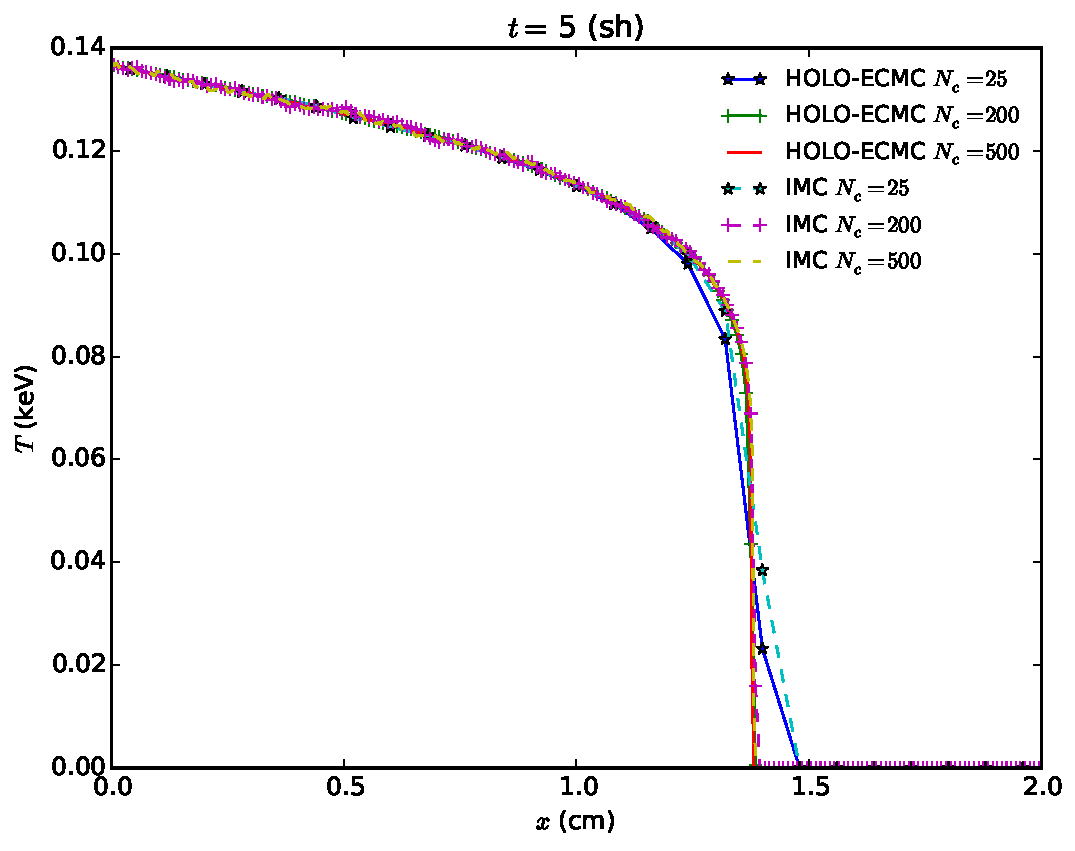
\includegraphics[width=0.99\linewidth]{marshak_mesh_conv.pdf}
    \caption{\label{marshak_mesh_conv} Convergence of IMC and HOLO-ECMC solutions.}
\end{subfigure}
\begin{subfigure}{0.5\textwidth}
  \centering
  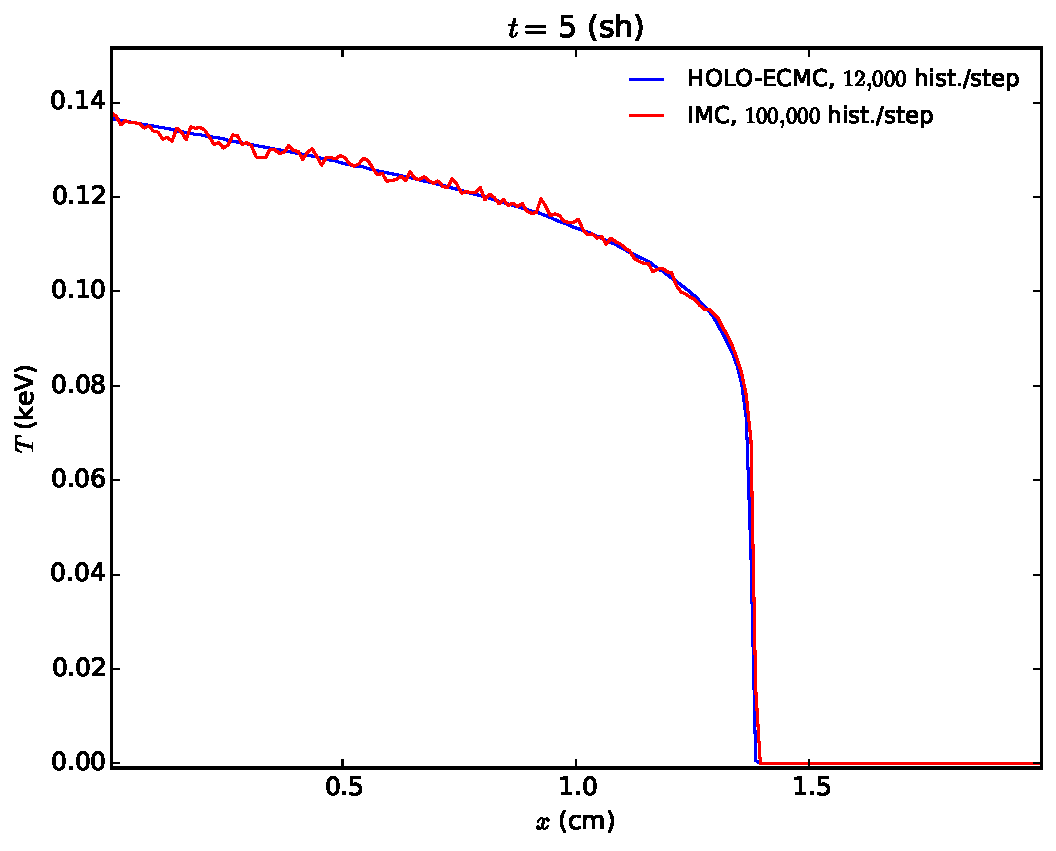
\includegraphics[width=0.99\linewidth]{marshak_200_compare.pdf}
  \caption{\label{marshak_200_compare}  Comparison of solutions for 200 spatial cells. }
\end{subfigure}
\caption{\bf Comparison of solutions for Marshak wave problem at $\mathbf{t=5}$ sh.}
\end{figure}

Fig.~\ref{marshak_mesh_conv} compares the cell-averaged radiation temperatures  for the
IMC and HOLO method with ECMC, for various number of spatial mesh cells $N_c$.  For the HOLO solver, we have used
4 equal-sized cells in $\mu$ for the finite-element angular mesh used by the ECMC solver. For the cases
of $N_c=25$ and $N_c=200$, 4,000 histories per batch (12,000 per time step)  were used.  For $N_c=500$, 16,000 histories per batch were used due to increased number of cells that
need to be sampled.  For all IMC calculations, 10$^5$ histories per time step were used. The solutions agree as the mesh is converged.  There is
similar agreement in the location of the wave front due to the linear shape of the emission source over a cell.  The cells
at the wave front required use of the lumping-equivalent discretization during the LO
solve, resulting in strictly positive solutions.


Fig.~\ref{marshak_200_compare} compares solutions
for the case of 200 cells.  For the IMC solution $10^5$ histories per time step were
simulated; for the HOLO method only $4,000$ histories per batch
(12,000 per time step) were simulated. There is significant statistical noise in the IMC solution
compared to the HOLO solution.  The HOLO solution visually demonstrates no statistical noise.  The relatively small number of histories is possible
due to the residual formulation and the initial guess of $\tilde{I}^{n}$ for the
first HO solve.  Since the transport solve is only determining the change over the
time step, the statistical noise in the result is small relative to the magnitude of
$I^{n+1}$.  Also, the source sampling only places particles in cells where the residual is
large.  No particles are sampled in the equilibrium region out front of the wave. 

We have measured the total CPU time for simulations to provide a crude measure of the
computational cost.  Absolute comparisons in the computational cost of the two
methods are difficult to make. For instance, the IMC and HOLO methods are implemented
in different code infrastructures. Additionally, the HOLO method fully resolves
non-linearities at each time step, whereas IMC is using a single linearized step with
lagged opacities.  

Table~\ref{marshak_table} compares simulation CPU times for IMC and the HOLO method
with ECMC for different numbers of histories per time step.  Also given is one case
with an increased time step size.   The HOLO method does not scale with the number of
histories due to the fixed cost of the LO solver.  The cost of the LO solver is more
significant at 12,000 histories per time step where IMC takes less time, whereas at
$10^5$ histories the HOLO simulation takes less time.    The gain in efficiency of
the HOLO method over IMC would be significant if the large reduction in statistical
error, for the same number of histories, is considered.  Similar to the results
in~\cite{park}, as the time step size is increased to to 0.005 sh, the IMC method
increases in cost (per time step) more than the HOLO method. The increase in the IMC
simulation time with a larger time step is due to the increased amount of (expensive) effective scattering
events.   
\begin{table}[H]
\centering
\caption{\label{marshak_table} \textbf{Total CPU time required for the Marshak Wave problem for 200 $x$ cells.  Simulation end time is $\mathbf{t=5}$ sh.}}
\vspace{-0.1in}
	\begin{tabular}{|c|c|c|c|}\hline
Hists. per step & $\Delta t (sh)$ & IMC & HOLO-ECMC \\ \hline
10$^5$                    &   0.001	& 5190 s &	4003 s\\
$1.2\times10^4 $   &    0.001	& 635   s &	692 s \\
$1.2\times10^4$     &   0.005	& 303	  s &    179 s \\ \hline
\end{tabular}
\end{table}


\Subsection{Two Material Problem}

This problem consists of an optically thin (left) and an optically thick (right) material region,
with constant opacities.  The material properties are given in
Table~\ref{two_mat_props}.  Initially the radiation and material energies are in
equilibrium at a temperature of 0.05 keV.  An isotropic incident intensity of 0.500 keV
is applied at $x=0$ at $t=0$; the isotropic incident intensity on the right boundary is 0.05
keV.  The simulation is ran for 5 sh. For all HOLO simulations, we have used 8 equal-sized mesh cells in $\mu$.
\begin{table}[H]
        \caption{Material properties for two material problem\label{two_mat_props}}
\centering
        \begin{tabular}{|c|cc|}  \cline{2-3}
            \multicolumn{1}{c|}{}   & $x \in [0,0.5)$ cm & $x \in [0.5,1.0]$ cm   \\ \hline
            $\sigma_a$ (cm$^-1$)  & 0.2 & 2000 \\
            $\rho$ (g cm$^-3$) & 0.01 & 10.0 \\
            $c_v$ (jks/keV-g) & $0.1$ & $0.1$ \\ \hline
        \end{tabular}
\end{table}
Fig.~\ref{twomat_full} compares the HOLO and IMC radiation 
temperatures at the end of the simulation. The IMC method used 10$^5$ histories per
time step, where as the HOLO method used $3\times10^4$ histories per time step.  The
IMC and HOLO results show good agreement
over the finer mesh.
On the coarse mesh ($N_c=20$), the HOLO method predicts the location of the
wave-front more accurately than the IMC method. 

Fig.~\ref{compare_ho} compares results for different HO solvers.  The HOLO algorithm
with the ECMC HO solver (HOLO-ECMC) results
are for running 3 batches of 10,000 histories, per time step. The solution for the HOLO method with a standard MC solver as the HO solver
(HOLO-SMC) with standard source sampling uses 10$^5$ histories per time step. Also
plotted is an S$_2$ solution obtained by using consistency terms that are equivalent
to S$_2$ and not performing the HO correction step.  The HOLO-SMC solution demonstrates significant
statistical noise.  This noise is introduced into the LO solver by bad statistics in
computing the consistency terms. The S$_2$ solution results in an artificially fast
wave front as expected, demonstrating the necessity of HO correction in this problem.

Total CPU times for the two material problem are given in Table~\ref{twomat_table}. The end time for the simulations in this table was reduced to 2 sh.  The observed behavior in the computational times is similar to those
in the first problem.  Because the opacities do not have a $T^{-3}$ behavior in this problem, the cost of the effective scattering cross section in IMC is more apparent, resulting in longer simulation times.  As the time step size is increased by a factor of 5, the average cost per time step for the simulation increases by a factor of $\sim3.4$; for HOLO-ECMC the increase is only $\sim1.1$.   
\begin{table}[htb!]
\centering
\caption{\label{twomat_table} \textbf{Total CPU time required for the two material problem.  Simulation end time is $\mathbf{t=2}$ sh.}}
	\begin{tabular}{|c|c|c|c|} \hline
Hists. per step & $\Delta t (sh)$ & IMC & HOLO-ECMC \\ \hline
10$^5$                    &   0.001	& 3428  &	673 \\
$3\times10^4 $   &    0.001	& 1036  &	397  \\
$3\times10^4$     &   0.005	&  699  &       86     \\ \hline
\end{tabular}
\end{table}





\begin{figure}
\begin{subfigure}{0.5\textwidth}
    \centering
    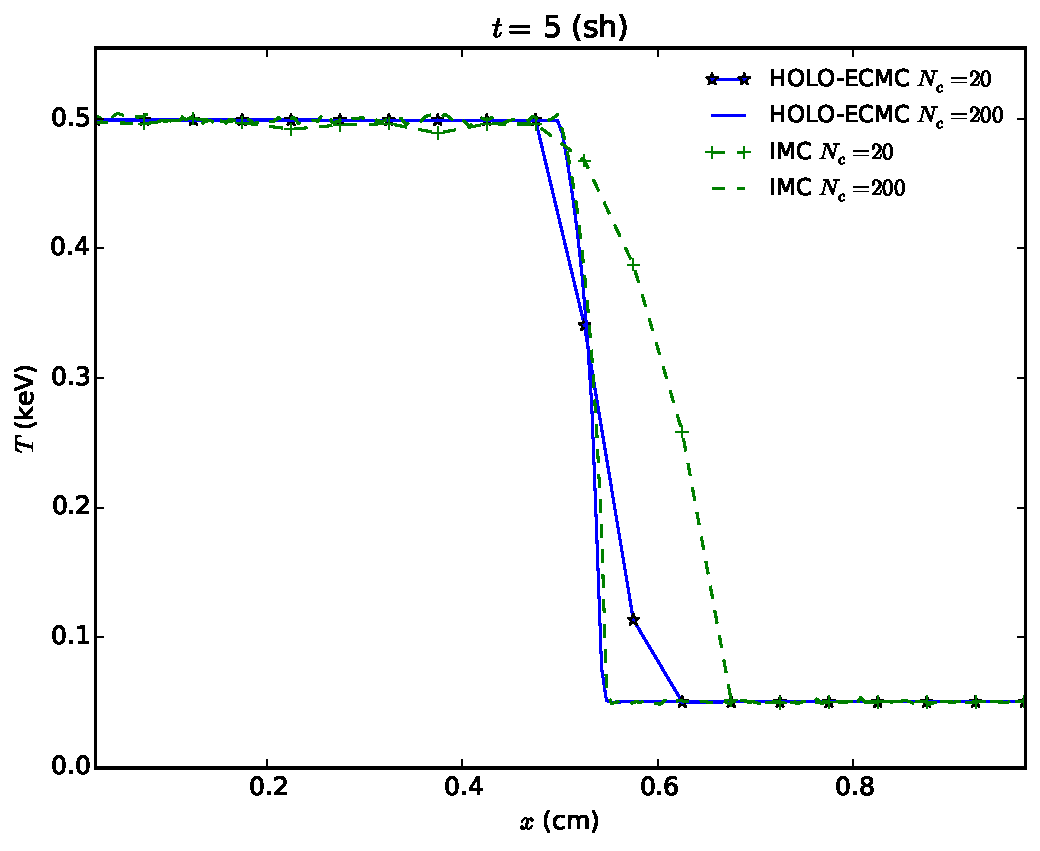
\includegraphics[width=0.99\textwidth]{two_mat_conv.pdf}
    \caption{Comparison of IMC and HOLO-ECMC.\label{twomat_full}}
\end{subfigure}    \begin{subfigure}{0.5\textwidth}
\centering
    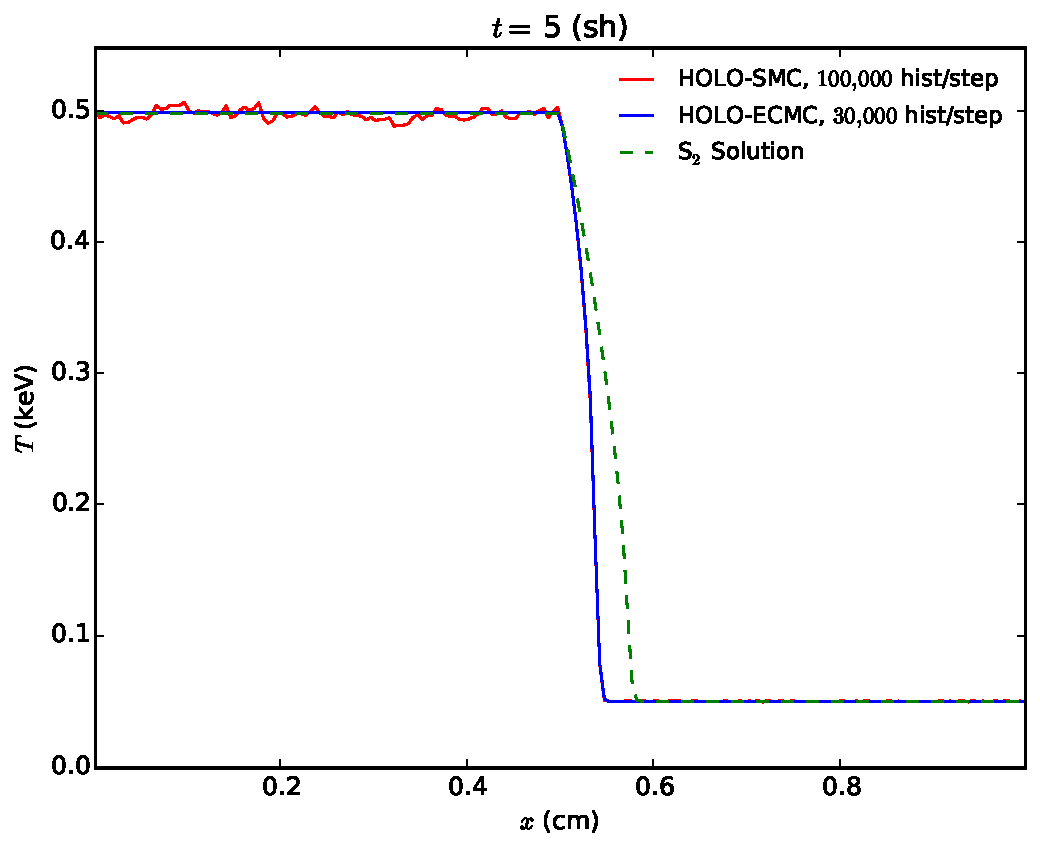
\includegraphics[width=0.99\textwidth]{two_mat_ho_compare.pdf}
    \caption{Comparison of SMC and ECMC HO solvers. \label{compare_ho}}
\end{subfigure}
    \caption{\bf Comparison of radiation temperatures for two material problem. \label{twomat}}
\end{figure}


\Section{Conclusions}

\Subsection{Summary}

We have been able to produce solutions for Marshak wave test problems using
a new HOLO method that is in agreement with IMC.  Unlike IMC, our method requires no effective scattering
events to be included in the MC simulation, limiting the total run time of the
simulations.  The LD spatial representation
mitigates issues with teleportation error, similar to source tilting in the IMC
algorithm.   The LO solver resolves the non-linearities in the equations resulting in a fully
implicit time discretization.  The ECMC approach, with initial guesses based on the
previous radiation intensity, results in efficient reduction of statistical error and
allows for particles to be distributed to largely varying regions of the problem.
The LO solver
can accurately and efficiently resolve the solution in diffusive regions, while the HO
transport solver provides the accuracy of a full transport treatment where necessary. 

The primary difficulty to overcome in the HO
solver is at the wave front.  A strictly positive functional representation of the angular flux
needs to be enforced for accurate solutions near the wave front.  The representation needs to be implemented
such that the spatial closure in the LO system is consistent with the HO
representation for the solution.  The ability to represent the solution accurately in
rapidly varying regions of the problem will be key for generalization of this method
to higher dimensions.  

\Subsection{Future Work} 

Future work will include comparisons of the HOLO method with IMC using a figure of
merit to quantify the efficiency of the simulations when statistical noise is
considered; the sensitivity of the method to mesh sizes and time step sizes will be
investigated more thoroughly.  The loss of accuracy in optically thin regions due to the time discretization of
the transport equation (which is required to form the residual in ECMC) will be
analyzed.  A formulazation of the ECMC method that allows for the trial space to be such that time-continous transport can
be treated with Monte Carlo is currently being investigated; the additional sampling
of the time variable will likely result in additional histories for problems where
the time change is great over a time step.  However, greater time accuracy is not of primary concern as this method isintended for use in
regions of high absorption-reemission where the LO acceleration is critical.

Ultimately, we plan to extend this method to multiple spatial dimensions for the 
case of multigroup TRT equations.  For TRT problems, it is important that
the LO spatial discretization satisfies the equilibirium diffusion limit.  To extend
to higher dimensions, our LD FE representation may require the use of a higher-degree
spatial representation for the LO system to achieve the diffusion
limit.  We will also
investigate the possibility of using the HO MC solution to provide cell inflows such
that the LO system correctly achieves the diffusion
limit.  Further asymptotic
analysis on the method will be applied before implementation.    It may be necessary to use a different LO system (e.g., the non-linear diffusion
acceleration approach in~\cite{rmc}), if the S$_2$-like equations become too
inefficient or difficult to implement in higher dimensions.  Alternatively, a
variable Eddington Tensor approach may provide more stability in rapidly variable
regions of the problem while still being
efficiently solved.

\section*{ACKNOWLEDGEMENTS}

This research was performed using funding received from the DOE Office of Nuclear
Energy's Nuclear Energy University Programs and under Los Alamos National Security,
LLC, for the National Nuclear Security Administration of the U.S. Department of
Energy under contract DE-AC52-06NA25396. 


\setlength{\baselineskip}{12pt}
%\Section*{REFERENCES}
\bibliographystyle{ans}
\bibliography{references}

\appendix

\section{Implementation of ECMC Tallies}

The HOLO algorithm uses a finite element representation in space and angle.  Over the
$i$-th spatial and $j$-th angular cell, the linear representation is defined as
\begin{equation}
    \tilde I(x,\mu) = I_a + I
\end{equation}
for $x_\il <  x \leq x_\ir$ and $\mu_\jl \leq \mu \leq \mu_\jr$ where indices have
been supressed for clarity and $I_a$ is the cell average intensity and $I_\mu$ and $I_x$ are
the first moment in $\mu$ and $x$, respectively.  Standard upwinding is used to
define the inflow at $x_{i-1/2}$. This representation can directly be plugged into
Eq.~\eqref{eq:resid} and evaluated to produce the source in the ECMC HO transport
problem.  

During the MC simulation, a projection of the error in the current estimate of
$\tilde{I}(x,\mu)$ is computed.  To project onto the LD FE trial space requires spatial and angular
moments of the angular intensity to be tallied. For instance, the first 
moment in $x$ of the $i$-th spatial and $j$-th angular cell is defined as
\begin{equation}
    I_{x,ij} = \frac{6}{h_xh_\mu}\int\limits_{\mu_{j-1/2}}^{\mu_{j+1/2}}
    \int\limits_{x_{i-1/2}}^{x_{i+1/2}} \left(\frac{x - x_i}{h_{x_i}}\right)
    I(x,\mu) \d x \d \mu.
\end{equation}
The $\mu$ moment and the moments of the intensity $I_a$, $I_\mu$, and $I_x$ are
all defined analagously. The tally estimator is defined by integrating along each
path in the cell as
\begin{equation}
    I_{x,ij} \simeq \frac{1}{h_xh_\mu} \int_{\Delta s_l}  w_l(x,\mu) \d s
\end{equation}
where $w(x,\mu)$ is the normalized weight in the MC simulation. Substituting the
exponential attenuation of the weight produces the result for this tally as
\begin{equation}
    I_{x,ij} \simeq \frac{1}{h_x h_\mu} DERP.
\end{equation}
The tally for the first moment in $\mu$ is 
\begin{equation}
    I_{\mu,ij} \simeq \frac{6}{h_x h_\mu}\sum_{l=1}^N \frac{\mu - \mu_j}{h_\mu}
        1 - exp\left( \sigma_t s \right)
\end{equation}
where $s$ is the path length of the track within the cell of interest.

\end{document}


